\documentclass[12pt,letterpaper]{report}\usepackage{graphicx, color}
%% maxwidth is the original width if it is less than linewidth
%% otherwise use linewidth (to make sure the graphics do not exceed the margin)
\makeatletter
\def\maxwidth{ %
  \ifdim\Gin@nat@width>\linewidth
    \linewidth
  \else
    \Gin@nat@width
  \fi
}
\makeatother

\IfFileExists{upquote.sty}{\usepackage{upquote}}{}
\definecolor{fgcolor}{rgb}{0.2, 0.2, 0.2}
\newcommand{\hlnumber}[1]{\textcolor[rgb]{0,0,0}{#1}}%
\newcommand{\hlfunctioncall}[1]{\textcolor[rgb]{0.501960784313725,0,0.329411764705882}{\textbf{#1}}}%
\newcommand{\hlstring}[1]{\textcolor[rgb]{0.6,0.6,1}{#1}}%
\newcommand{\hlkeyword}[1]{\textcolor[rgb]{0,0,0}{\textbf{#1}}}%
\newcommand{\hlargument}[1]{\textcolor[rgb]{0.690196078431373,0.250980392156863,0.0196078431372549}{#1}}%
\newcommand{\hlcomment}[1]{\textcolor[rgb]{0.180392156862745,0.6,0.341176470588235}{#1}}%
\newcommand{\hlroxygencomment}[1]{\textcolor[rgb]{0.43921568627451,0.47843137254902,0.701960784313725}{#1}}%
\newcommand{\hlformalargs}[1]{\textcolor[rgb]{0.690196078431373,0.250980392156863,0.0196078431372549}{#1}}%
\newcommand{\hleqformalargs}[1]{\textcolor[rgb]{0.690196078431373,0.250980392156863,0.0196078431372549}{#1}}%
\newcommand{\hlassignement}[1]{\textcolor[rgb]{0,0,0}{\textbf{#1}}}%
\newcommand{\hlpackage}[1]{\textcolor[rgb]{0.588235294117647,0.709803921568627,0.145098039215686}{#1}}%
\newcommand{\hlslot}[1]{\textit{#1}}%
\newcommand{\hlsymbol}[1]{\textcolor[rgb]{0,0,0}{#1}}%
\newcommand{\hlprompt}[1]{\textcolor[rgb]{0.2,0.2,0.2}{#1}}%

\usepackage{framed}
\makeatletter
\newenvironment{kframe}{%
 \def\at@end@of@kframe{}%
 \ifinner\ifhmode%
  \def\at@end@of@kframe{\end{minipage}}%
  \begin{minipage}{\columnwidth}%
 \fi\fi%
 \def\FrameCommand##1{\hskip\@totalleftmargin \hskip-\fboxsep
 \colorbox{shadecolor}{##1}\hskip-\fboxsep
     % There is no \\@totalrightmargin, so:
     \hskip-\linewidth \hskip-\@totalleftmargin \hskip\columnwidth}%
 \MakeFramed {\advance\hsize-\width
   \@totalleftmargin\z@ \linewidth\hsize
   \@setminipage}}%
 {\par\unskip\endMakeFramed%
 \at@end@of@kframe}
\makeatother

\definecolor{shadecolor}{rgb}{.97, .97, .97}
\definecolor{messagecolor}{rgb}{0, 0, 0}
\definecolor{warningcolor}{rgb}{1, 0, 1}
\definecolor{errorcolor}{rgb}{1, 0, 0}
\newenvironment{knitrout}{}{} % an empty environment to be redefined in TeX

\usepackage{alltt}
\renewcommand{\familydefault}{\sfdefault}
\newcommand{\factoid}[1]{\flushleft{\large{#1}}}
\newenvironment{itemize*}%
  {\begin{itemize}%
    \setlength{\itemsep}{0pt}%
    \setlength{\parskip}{0pt}}%
  {\end{itemize}}
\usepackage[font=sf]{floatrow}
%\usepackage[font = sf]{caption}
\restylefloat{table}
%\usepackage[utf8]{inputenc}
\usepackage{siunitx,booktabs}

\sisetup{
    group-digits=true,
    group-separator={\,},
}
\usepackage{graphicx}
\usepackage{lipsum}
%\usepackage{titlesec}
\begin{document}





{\flushleft   
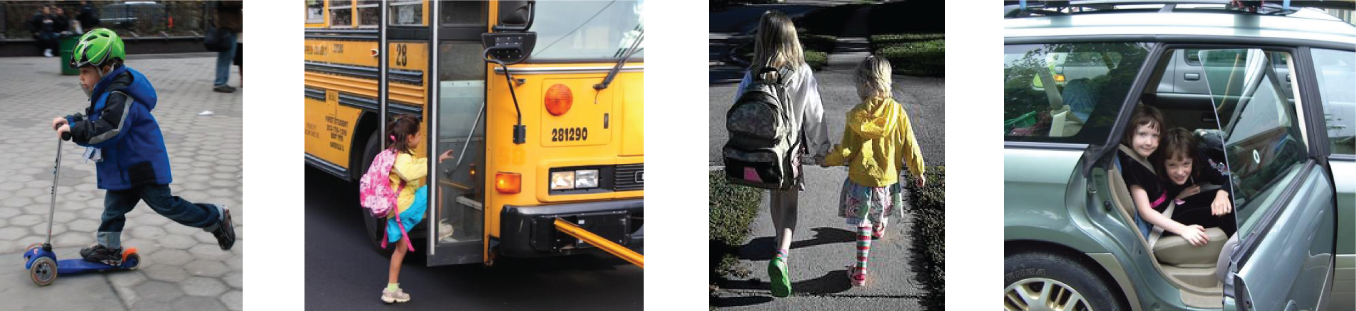
\includegraphics[height=32 mm]{KidsAreCommutersToo_TitleImage}
  {
    MySchoolCommute.org\\
    Survey Report\\
    % Survey Report\\[.2 cm]
    Lawrence - Alexander B Bruce\\ 
  }                                 
\today \\     
}

\section*{Introduction}
This report will help your school plan safe transportation options for all students. It contains the results of a survey conducted at Lawrence - Alexander B Bruce from \emph{first month}, \emph{first year} to \emph{last month}, \emph{last year}. Participating parents provided information about how students travel to school and their approximate home location. If your school is interested in 
\begin{itemize*}
\item reducing traffic congestion,
\item encouraging walking and biking,
\item increasing safety, or
\item tracking progress towards community goals,
\end{itemize*}
then this information can help you identify the right strategies and best opportunities 
for new projects and investments. 

\subsection*{How to Read This Report}
This report measures distance to school in terms of walksheds and bikesheds. A \emph{walkshed} includes all the homes within a certain distance to school, based on mapped sidewalks, pedestrian paths, and low volume roadways. We define walksheds for 0.5, 1.0, and 1.5 mile walking distances to school. A \emph{bikeshed} of 2.0 miles also includes multi-use paths and on-road cycle facilities, where mapped. For a map of the walksheds and bikesheds, see the back cover or last page of the report. Where "walkshed" is used alone, it always includes the bikeshed of the same distance.
\newpage
\section*{Survey Statistics}
{\factoid Survey Dates: \emph{Beginning Date} to \emph{End date}}
{\factoid Responses Received: 251}
{\factoid School-wide Participation Rate: 46\%}

\begin{knitrout}
\definecolor{shadecolor}{rgb}{0.969, 0.969, 0.969}\color{fgcolor}\begin{figure}[H]


{\centering 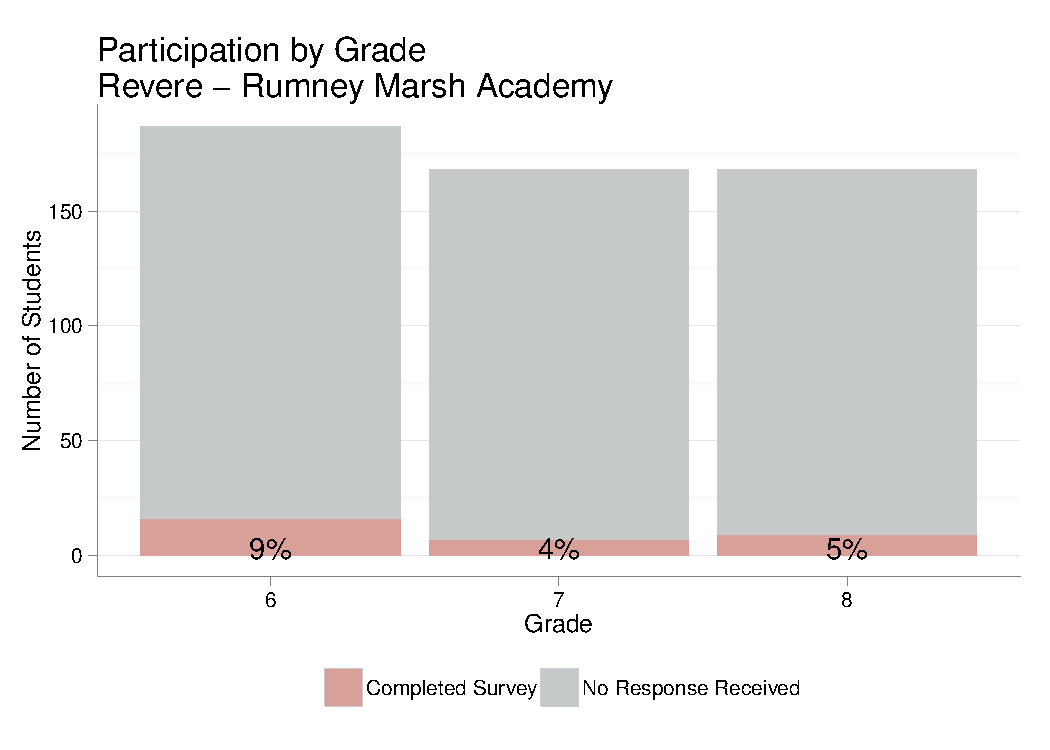
\includegraphics[width=\maxwidth]{figure/g_dfg} 

}

\caption[Labels show participation rate for each grade]{Labels show participation rate for each grade. Total enrollment (Completed + No Response) is current as of October, 2013, per Department of Elementary and Secondary Education.\label{fig:g_dfg}}
\end{figure}


\end{knitrout}


Survey responses from each grade were used to estimate the distance and travel choice for the entire grade.The higher the participation rate, the more reliable the survey results are.

\newpage
\section*{Student Proximity}
{\factoid Average Distance to School: 0.9 miles}
{\factoid Percent within 1.0 Mile Walkshed: 60\%}
{\factoid Percent within 2.0 Mile Bikeshed: 97\%}
\begin{figure}[H]


{\centering 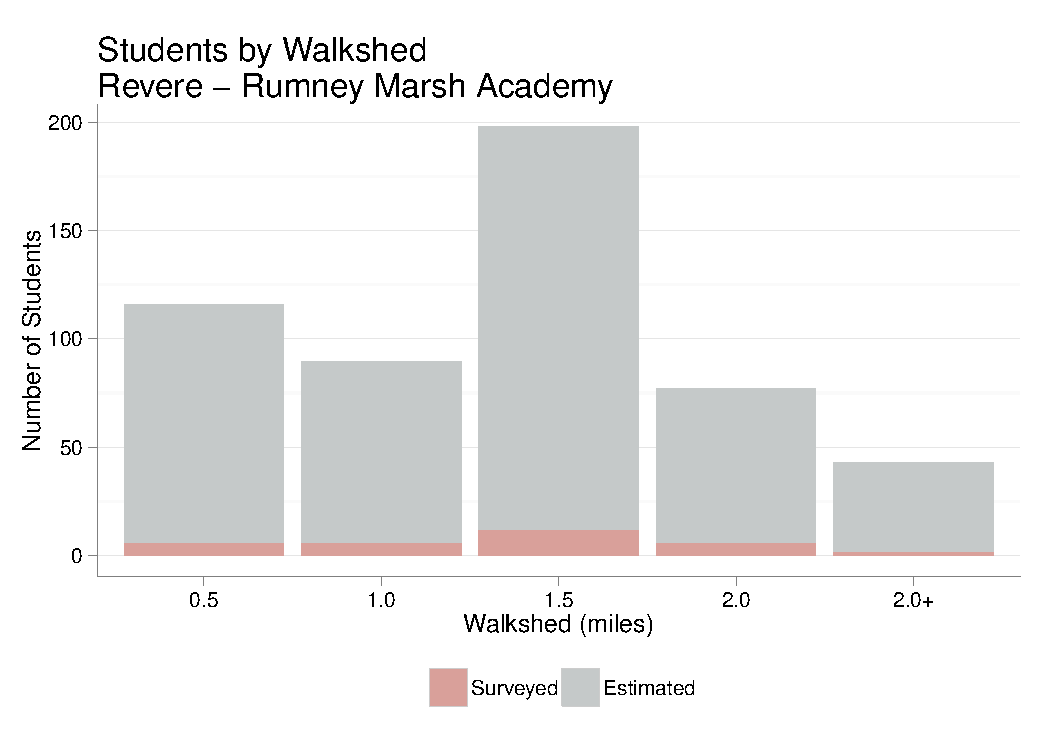
\includegraphics[width=\maxwidth]{figure/b_dfg} 

}

\caption[Surveyed and Estimated Student Totals by Walkshed]{Surveyed and Estimated Student Totals by Walkshed\label{fig:b_dfg}}
\end{figure}




% latex.default(b_dft, file = "", headings = c("", buffers), first.hline.double = FALSE,      rowname = NULL, where = "H", col.just = c("l", rep("r", 5)),      caption = "Surveyed and Estimated Total Students by Walkshed") 
%
\begin{table}[H]
\caption{Surveyed and Estimated Total Students by Walkshed\label{b}} 
\begin{center}
\begin{tabular}{lrrrrr}
\hline
\multicolumn{1}{c}{}&\multicolumn{1}{c}{0.5}&\multicolumn{1}{c}{1.0}&\multicolumn{1}{c}{1.5}&\multicolumn{1}{c}{2.0}&\multicolumn{1}{c}{2.0+}\tabularnewline
\hline
Estimated Total&212&111&142&58&18\tabularnewline
Surveyed Students&99&50&63&30&9\tabularnewline
Percent of Students&39\%&21\%&26\%&11\%&3\%\tabularnewline
\hline
\end{tabular}
\end{center}
\end{table}




\newpage
\section*{Student Travel Choices}
{\factoid Percent of Trips Made by Car: 46\%}
{\factoid Percent of Trips Made by Walking\textbackslash Biking: 29\%}
\newline
{\flushleft The chart below shows what percent of trips are made by each travel mode in the morning and afternoon.}

\begin{knitrout}
\definecolor{shadecolor}{rgb}{0.969, 0.969, 0.969}\color{fgcolor}\begin{figure}[H]


{\centering 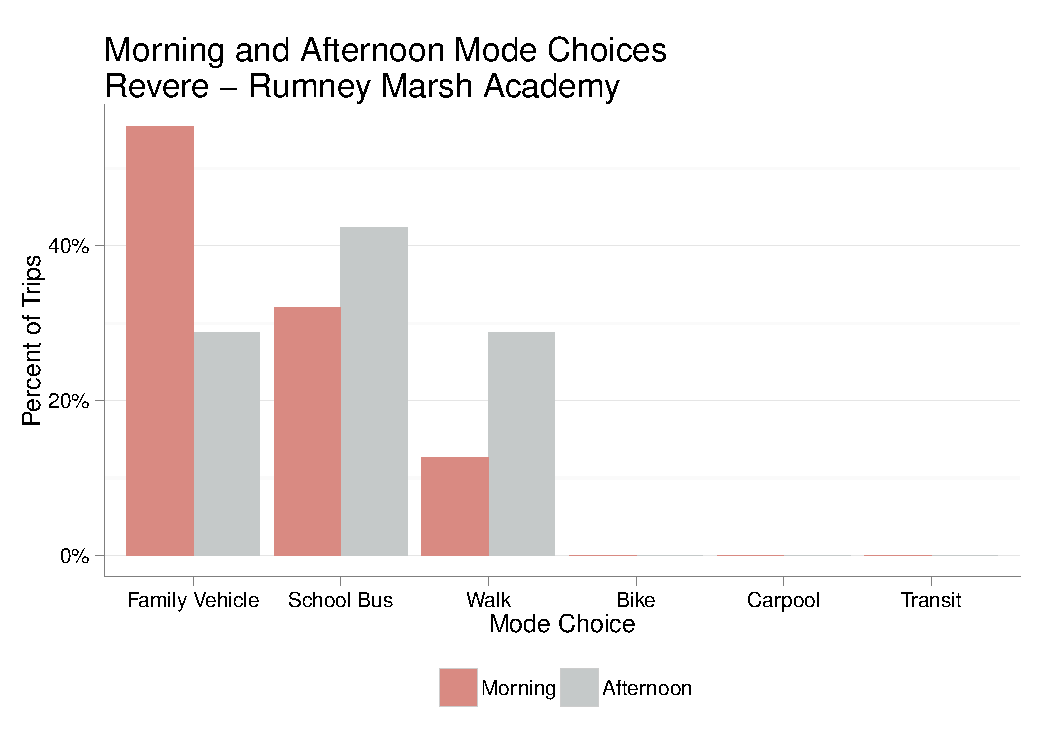
\includegraphics[width=\maxwidth]{figure/modeByTime} 

}

\caption[Mode share estimates are based on responses received for each grade]{Mode share estimates are based on responses received for each grade.\label{fig:modeByTime}}
\end{figure}


\end{knitrout}


Walk share is higher in the afternoon than it is in the evening: 
34.5\% versus 23.8\%. The auto share is lower in the afternoon, indicating that as many as 28.9\% of those who are driven to school in the morning get home by other means in the afternoon.


\begin{knitrout}
\definecolor{shadecolor}{rgb}{0.969, 0.969, 0.969}\color{fgcolor}

{\centering 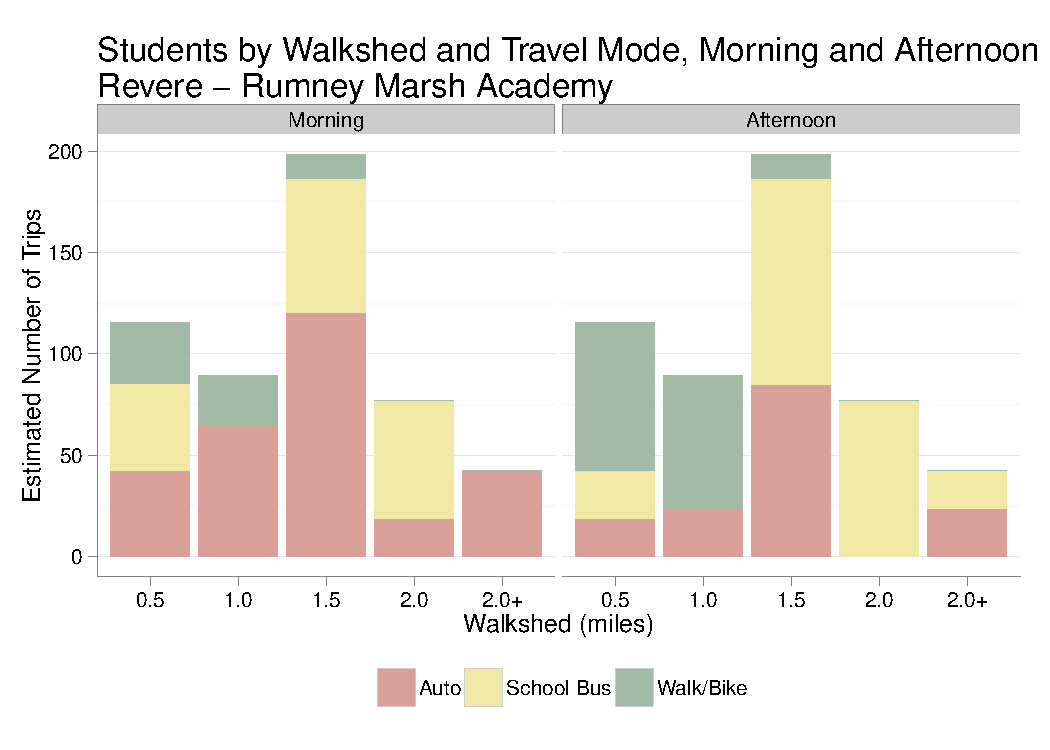
\includegraphics[width=\maxwidth]{figure/mByBuffer} 

}



\end{knitrout}


% latex.default(mSb_df_wide, file = "", cgroup = c("", "Trips by Walkshed",      "Percents"), n.cgroup = c(1, 5, 5), first.hline.double = FALSE,      rowname = NULL, where = "!htbp", col.just = c("l", rep("r",          10))) 
%
\begin{table}[!htbp]
\begin{center}
\begin{tabular}{lcrrrrrcrrrrr}
\hline
\multicolumn{1}{c}{\bfseries }&\multicolumn{1}{c}{\bfseries }&\multicolumn{5}{c}{\bfseries Trips by Walkshed}&\multicolumn{1}{c}{\bfseries }&\multicolumn{5}{c}{\bfseries Percents}\tabularnewline
\cline{1-13}
\multicolumn{1}{c}{}&\multicolumn{1}{c}{}&\multicolumn{1}{c}{0.5}&\multicolumn{1}{c}{1.0}&\multicolumn{1}{c}{1.5}&\multicolumn{1}{c}{2.0}&\multicolumn{1}{c}{2.0+}&\multicolumn{1}{c}{}&\multicolumn{1}{c}{0.5}&\multicolumn{1}{c}{1.0}&\multicolumn{1}{c}{1.5}&\multicolumn{1}{c}{2.0}&\multicolumn{1}{c}{2.0+}\tabularnewline
\hline
Auto&&122&46&84&26&16&&58\%&41\%&59\%&45\%&86\%\tabularnewline
School Bus&&33&30&29&24&3&&16\%&27\%&20\%&42\%&14\%\tabularnewline
Walk&&56&36&29&8&0&&27\%&32\%&20\%&14\%&0\%\tabularnewline
Total&&212&111&142&58&18&&100\%&100\%&100\%&100\%&100\%\tabularnewline
\hline
\end{tabular}
\end{center}
\end{table}




% # 
% # <<modeDFMorningWideTable, echo=FALSE,fig.width=7,fig.height=5,fig.align="center",fig.pos='H',results="asis">>=
% # @
% 
% busEligibleDrivenPct\% of students who are "Bus Eligible" are currently being driven to school, generating busEligibleDrivenCount drop-offs each morning.
% 
\newpage
\section*{Greenhouse Gas Emissions}
{\factoid Per-student GHG emissions within one mile: 102 kg}
{\factoid Per-student GHG emissions beyond one mile: 363 kg}

% latex.default(ghgBufferDFgeneric[c("Buffer", "studentsEst", "ghgEst",      "ghgEstPerCap", "PctTotGHGprint")], file = "", colheads = c("Buffer",      "Students", "Total GHG", "GHG Per Capita", "Percent Total GHG"),      where = "H", first.hline.double = FALSE, caption = paste("GHG Emissions by Walkshed, ",          paste(School_Name, ".", sep = "")), col.just = c("l",          rep("r", 4)), rowname = NULL) 
%
\begin{table}[H]
\caption{GHG Emissions by Walkshed,  Lawrence - Alexander B Bruce.\label{ghgBufferDFgeneric}} 
\begin{center}
\begin{tabular}{lrrrr}
\hline
\multicolumn{1}{c}{Buffer}&\multicolumn{1}{c}{Students}&\multicolumn{1}{c}{Total GHG}&\multicolumn{1}{c}{GHG Per Capita}&\multicolumn{1}{c}{Percent Total GHG}\tabularnewline
\hline
0.5&220&14338&65&13\%\tabularnewline
1.0&105&18658&178&17\%\tabularnewline
1.5&130&31579&243&28\%\tabularnewline
2.0&67&32398&484&29\%\tabularnewline
2.0+&19&14536&765&13\%\tabularnewline
\hline
\end{tabular}
\end{center}
\end{table}



% 
\section*{How Your School Compares}
% latex.default(pSaggLatex, file = "", colheads = c("", "Percent Within 1 Mile",      "1.0 Mile Walk Share", "GHG Per Student"), where = "H", first.hline.double = FALSE,      caption = paste("1.0 Mile walk share and GHG emissions: ",          School_Name, " versus peer schools. Peer schools are those \n                                         whose share of students within 1.0 mile of \n                                         school is within 10\\% of the share at your \n                                         school.",          sep = ""), col.just = c("l", rep("r", 3)), rowname = NULL) 
%
\begin{table}[H]
\caption{1.0 Mile walk share and GHG emissions: Lawrence - Alexander B Bruce versus peer schools. Peer schools are those 
                                         whose share of students within 1.0 mile of 
                                         school is within 10\% of the share at your 
                                         school.\label{pSaggLatex}} 
\begin{center}
\begin{tabular}{lrrr}
\hline
\multicolumn{1}{c}{}&\multicolumn{1}{c}{Percent Within 1 Mile}&\multicolumn{1}{c}{1.0 Mile Walk Share}&\multicolumn{1}{c}{GHG Per Student}\tabularnewline
\hline
Your School&60\%&29\%&206\tabularnewline
Peer Schools&56\%&27\%&253\tabularnewline
\hline
\end{tabular}
\end{center}
\end{table}




% 
% 
% <<modeByBufferTableAllSchools, echo=FALSE, eval=TRUE, results="asis",comment="Counts and percentages of student travel mode by walkshed." >>=
% @
% 
% 
% \emph{High student proximity is a prerequisite to having a high walk/bike share, but not a guarantee.} Comparison of schoolwide walk/bike share to student proximity identified three general categories of schools which differ in their walk to school and mode shift potential.  In the \emph{High Proximity, High Walk Share} schools, more than 75\% of students live within a mile of school and walk rates exceed 30\%. The \emph{Untapped Walk Potential} schools have similar student proximity but much lower walk rates, suggesting the possibility of substantial mode shift (10 - 20\%) through SRTS programs. The \emph{Dispersed Enrollment, Limited Walk Potential} schools are those where fewer than 60\% of students live within a mile of school; as a result, the schoolwide walk rates rarely exceed 21\%. 
% 
% TypeParagraph
% 
% <<walkPotentialPlot, echo=FALSE,fig.width=7,fig.height=5,fig.align="center",fig.pos='H',fig.cap="Red indicates dispersed enrollment, limited walk potential; yellow indicates untapped walk potential; green indicates high proximity, high walk share.">>=
% @
% 
% \subsection*{Mode Choice and Time of Day}
% How students travel to and from school can depend on the time of day. At previously surveyed schools, 50\% of morning trips were family vehicle, non-carpool trips, versus 43\% of afternoon trips. At School_Name, famVehMorningPct\% of morning trips are family vehicle, non-carpool, versus famVehAfternoonPct\% of trips in the afternoon.
% 
% <<modeByTime, echo=FALSE,fig.width=7,fig.height=5,fig.align="center",fig.pos='H'>>=
% @
% 
% Trip chaining can have a strong influence on the divergence of morning and afternoon mode choice. At other schools, 70\% of morning auto trips (family vehicle and carpool) are made by parents who continue on to work or another destination. There are about 7\% fewer auto trips in the afternoon, but this difference appears to be the result of fewer parents picking up their children on the way home from work. In the afternoon, the percentage of auto trips that are en route drops to 64\%.
% 
% At School_Name, autoMorningPct\% of morning trips are by automobile, versus autoAfternoonPct\% of afternoon trips. Enroute trips comprise enRouteMorningPct\% of automobile trips in the morning, and enRouteAfternoonPct\% of trips in the afternoon.
% 
% <<chainByTime, echo=FALSE,fig.width=7,fig.height=5,fig.align="center",fig.pos='H'>>=
% @
% 
% \subsection*{Mode Choice and Vehicle Availability}
% Vehicle availability can also influence mode choice. lowVehicleHHsPct\% of survey responses from School_Name indicated that there were more licensed drivers than vehicles in the household or no vehicles at all. Vehicle availability is considered to be low in these households. Among these households, lowVehicleWalkPctTo\% and lowVehicleWalkPctFrom\% of students walk, bike, or take the bus to and from school in the morning and afternoon, respectively. Among students in high vehicle available households, the corresponding numbers are highVehicleWalkPctTo\% and highVehicleWalkPctFrom\%.
% 
% <<ChainByTimeAndAvail,  echo=FALSE, eval=TRUE, results="asis">>=
% @
% 
% 
% \section*{GHG Emissions}
% Students who live farther from school tend to emit more green house gases (GHGs) than students who live closer to school. From previous surveys, annual per-student GHG emissions among students who live more than 1.5 miles from school were 381 kilograms (kg) versus 66 kg for students within one-half mile, an almost six-fold increase. At School_Name, students who live more than 1.5 miles from school emit ghgPerCap15Buffer kgs per-capita per school year, versus ghgPerCap05Buffer kg for students within half a mile of school. 
% 
% <<ghgTableSchool,  echo=FALSE, eval=TRUE, results="asis">>=
% @
% 
% 
% <<ghgTableSchoolAllSch,  echo=FALSE, eval=TRUE, results="asis">>=
% @
\end{document}
